\documentclass[12pt]{article}
\usepackage[english]{babel}
\usepackage[utf8]{inputenc}

%% Pointer to 'default' preamble, other reusable files
% pacakages and definitions

\usepackage{geometry}
\geometry{
	letterpaper, 
	portrait, 
	top=.75in,
	left=.8in,
	right=.75in,
	bottom=.5in		} 	% Page Margins
	
%% additional packages for nice things
\usepackage{amsmath} 	% for most math
\usepackage{commath} 	% for abs
\usepackage{lastpage}	% for page count
\usepackage{amssymb} 	% for therefore
\usepackage{graphicx} 	% for image handling
\usepackage{wrapfig} 	% wrap figures
\usepackage[none]{hyphenat} % for no hyphenations
\usepackage{array} 		% for >{} column characterisctis
\usepackage{physics} 	% for easier derivative \dv....
\usepackage{tikz} 		% for graphic@!
\usepackage{circuitikz} % for circuits!
\usetikzlibrary{arrows.meta} % for loads
\usepackage[thicklines]{cancel}	% for cancels
\usepackage{xcolor}		% for color cancels
\usepackage[per-mode=fraction]{siunitx} % for si units and num
\sisetup{group-separator = {,}, group-minimum-digits = 3} % additional si unit table functionality

\usepackage{fancyhdr} 	% for header
\usepackage{comment}	% for ability to comment out large sections
\usepackage{multicol}	% for multiple columns using multicols
\usepackage[framed,numbered]{matlab-prettifier} % matlab sytle listing
\usepackage{marvosym} 	% for boltsymbol lightning
\usepackage{pdflscape} 	% for various landscape pages in portrait docs.
%\usepackage{float}
\usepackage{fancyvrb}	% for Verbatim (a tab respecting verbatim)
\usepackage{enumitem}	% for [resume] functionality of enumerate
\usepackage{spreadtab} 	% for using formulas in tables}
\usepackage{numprint}	% for number format in spread tab
\usepackage{subcaption} % for subfigures with captions
\usepackage[normalem]{ulem} % for strike through sout

% for row colors in tables....
\usepackage{color, colortbl}
\definecolor{G1}{gray}{0.9}
\definecolor{G2}{rgb}{1,0.88,1}%{gray}{0.6}
\definecolor{G3}{rgb}{0.88,1,1}

% For table formatting
\usepackage{booktabs}
\renewcommand{\arraystretch}{1.2}
\usepackage{floatrow}
\floatsetup[table]{capposition=top} % put table captions on top of tables

% Caption formating footnotesize ~ 10 pt in a 12 pt document
\usepackage[font={small}]{caption}

%% package config 
\sisetup{output-exponent-marker=\ensuremath{\mathrm{E}}} % for engineer E
\renewcommand{\CancelColor}{\color{red}}	% for color cancels
\lstset{aboveskip=2pt,belowskip=2pt} % for more compact table
%\arraycolsep=1.4pt\def
\setlength{\parindent}{0cm} % Remove indentation from paragraphs
\setlength{\columnsep}{0.5cm}
\lstset{
	style      = Matlab-editor,
	basicstyle = \ttfamily\footnotesize, % if you want to use Courier - not really used?
}
\renewcommand*{\pd}[3][]{\ensuremath{\dfrac{\partial^{#1} #2}{\partial #3}}} % for larger pd fracs
\renewcommand{\real}[1]{\mathbb{R}\left\{ #1 \right\}}	% for REAL symbol
\newcommand{\imag}[1]{\mathbb{I}\left\{ #1 \right\}}	% for IMAG symbol
\definecolor{m}{rgb}{1,0,1}	% for MATLAB matching magenta
	
%% custom macros
\newcommand\numberthis{\addtocounter{equation}{1}\tag{\theequation}} % for simple \numberthis command

\newcommand{\equal}{=} % so circuitikz can have an = in the labels
\newcolumntype{L}[1]{>{\raggedright\let\newline\\\arraybackslash\hspace{0pt}}m{#1}}
\newcolumntype{C}[1]{>{\centering\let\newline\\\arraybackslash\hspace{0pt}}m{#1}}
\newcolumntype{R}[1]{>{\raggedleft\let\newline\\\arraybackslash\hspace{0pt}}m{#1}}

%% Header
\pagestyle{fancy} % for header stuffs
\fancyhf{}
% spacing
\headheight 29 pt
\headsep 6 pt
%%% custom commands for nicer units
\newcommand{\mw}{\ensuremath{\text{ MW}}}
\newcommand{\hz}{\ensuremath{\text{ Hz}}}
\newcommand{\pu}{\ensuremath{\text{ Pu}}}
\newcommand{\sbase}{\ensuremath{\text{S}_{\text{Base}}}}
\newcommand{\fbase}{\ensuremath{f_{\text{Base}}}}
\newcommand{\mbase}[1]{\ensuremath{\text{M}_{\text{Base}_{#1}}}}
\newcommand{\hsys}{\ensuremath{\text{ H}_{\text{sys}}}}


%% Header
\rhead{Thad Haines \\ Page \thepage\ of \pageref{LastPage}}
\chead{Research Update \\ Week of February 24th, 2020}
\lhead{Research \\ }

%\usepackage{graphicx}
%\graphicspath{ {figures/} }
%\newcommand{\caseName}{ }

\begin{document}
\begin{multicols}{2}
\raggedright
	\paragraph{Thesis Schedule:}
	\begin{enumerate}
\itemsep0em 
		\item Revised thesis to Committee week of \\ \textbf{Mar 9} (pre-spring break).
		\item Thesis Defense week of \textbf{April 13}.
		\item Final thesis and docs to Southergill week of \textbf{April 20}.
\item Other tasks:
\subitem Complete other graduation forms
\subitem Book room for defense
\subitem Get EIT references
\end{enumerate}

	\paragraph{Recent Progress:}
	\begin{enumerate}
\itemsep0em 
\item Thesis `draft' sent to Southergill for format check. Apparently as long as the margins are 1", everything looks fine.
\item Thesis `draft' sent to Donnelly
\item Software documentation created from sections of thesis.
\item Definite Time Controller (DTC) Agent created and tested.
\item Modifiable system H tested
\item 12 machine system created
\item Initial WECC step frequency results

		\item GitHub updated:\\
		\verb|https://github.com/thadhaines/ |\\
(includes draft thesis and software docs)

\vfill\null
\columnbreak
	
	\end{enumerate}
\paragraph{Current Tasks:}
	\begin{enumerate}
		\itemsep0em 
		\item Test DTC capabilities with Governors
\begin{itemize}
			\item Given BPA issue is believed to be a step of governor Pref based on frequency deviation that occurs on a timer. i.e. $P_{ref} = P_{ref0} + \dfrac{\Delta \omega}{R}M_{base} $ every $x$ seconds.
			\item A simple six machine scenario is being built to show test this hypothesis.  
\end{itemize}

		\item Figure out how to do WECC data validation
\begin{itemize}
			\item .chf too big to load into MATLAB
			\item Python .mat file has issues being imported into MATLAB (too many nested structures?)
\end{itemize}

		\item Solidify test cases for engineering problem
\item Test `soft trip' where $ P = Q_{min}= Q_{max} = 0$.
\item Add ability to change Qmin/Qmax of PSLF system via PSLTDSim

		\item Update Code flowchart and finalize code% to aid in further development.
		\item Thesis work 

\end{enumerate}


\begin{comment}

\paragraph{Proposed MiniWECC test cases:} \ \\
duration: 4-6 hours
\begin{itemize}
	\itemsep0em 
\item system noise 
\item wind generation ramps 
\item daily load cycle (during peak/valley transition)
\end{itemize}

Control varaitions:\\
Normal gov deadband and large gov deadband \\
Fast (seconds) and slow (minutes) AGC
\\ Three cases: 
\begin{itemize}
	\itemsep0em 
\item normal gov, Slow AGC
\item normal gov, Fast AGC
\item large gov, Fast AGC
\end{itemize}

Experimental Measures:
\begin{itemize}
\itemsep 0em
\item Valve movement
\item NERC mandate adherence
\end{itemize}
\end{comment}
		%\item Keep Goals and Requests in mind.


	\paragraph{Current Questions:}
	\begin{enumerate}
\itemsep0em 
	\item BPA response to GDACs info request?
	\end{enumerate}
	


\begin{comment}
\paragraph{Future Tasks:} %(Little to No Progress since last time / Things coming down the pipe)
	\begin{enumerate}
		
		\item Add import mirror / bypass mirror init sequence option to prevent repeated mirror creations.

		\item Bring wind into simulation \\ (ramp ungoverned generators?)


		
	\end{enumerate}
\paragraph{Future Work: (not by me)}
\begin{itemize}
\item Find best/correct way to trip gens in PSLF from python.
\item Account for different types of loads better. (exponential load model) % read from dyd
\item Work to incorporate Matt's \emph{Suggested Use Cases} into simulation.
		\begin{itemize}
		\item Add Shunt Group Agent
		\item Work to Define Definite Time Controller user input
		\end{itemize} 


		\item Investigate ULTC action.

		\item Create an agent for every object: \\ ULTC, SVD, \ldots

		\item Move away from reliance on GE
		
\end{itemize}

\paragraph{Matt Requests:}
\begin{enumerate}
		\item Enable multiple dyd files to overwrite / replace previously defined agents/parameters
		\item Allow for variable time steps.
\end{enumerate}
\end{comment}

\vfill\null
\end{multicols}


\pagebreak
\paragraph{12 Machine} System is essentially the six machine system with twice as many generators.\\

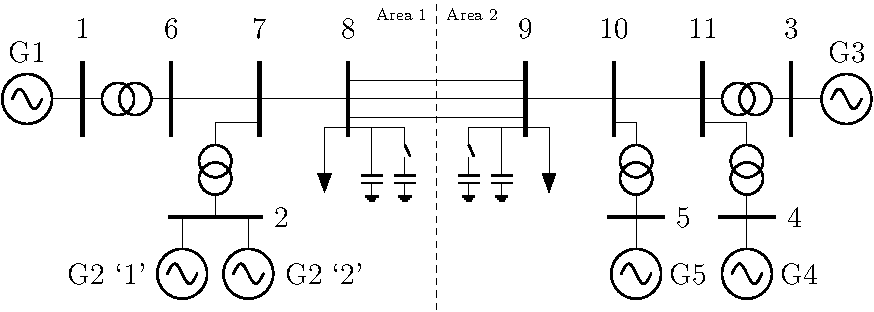
\includegraphics[width=\linewidth]{../../models/12machine/12Machine}

\paragraph{WECC step Results} Due to data issues, a more `get er done' approach was taken to depict the frequency output from PSDS and LTD on top of each other.

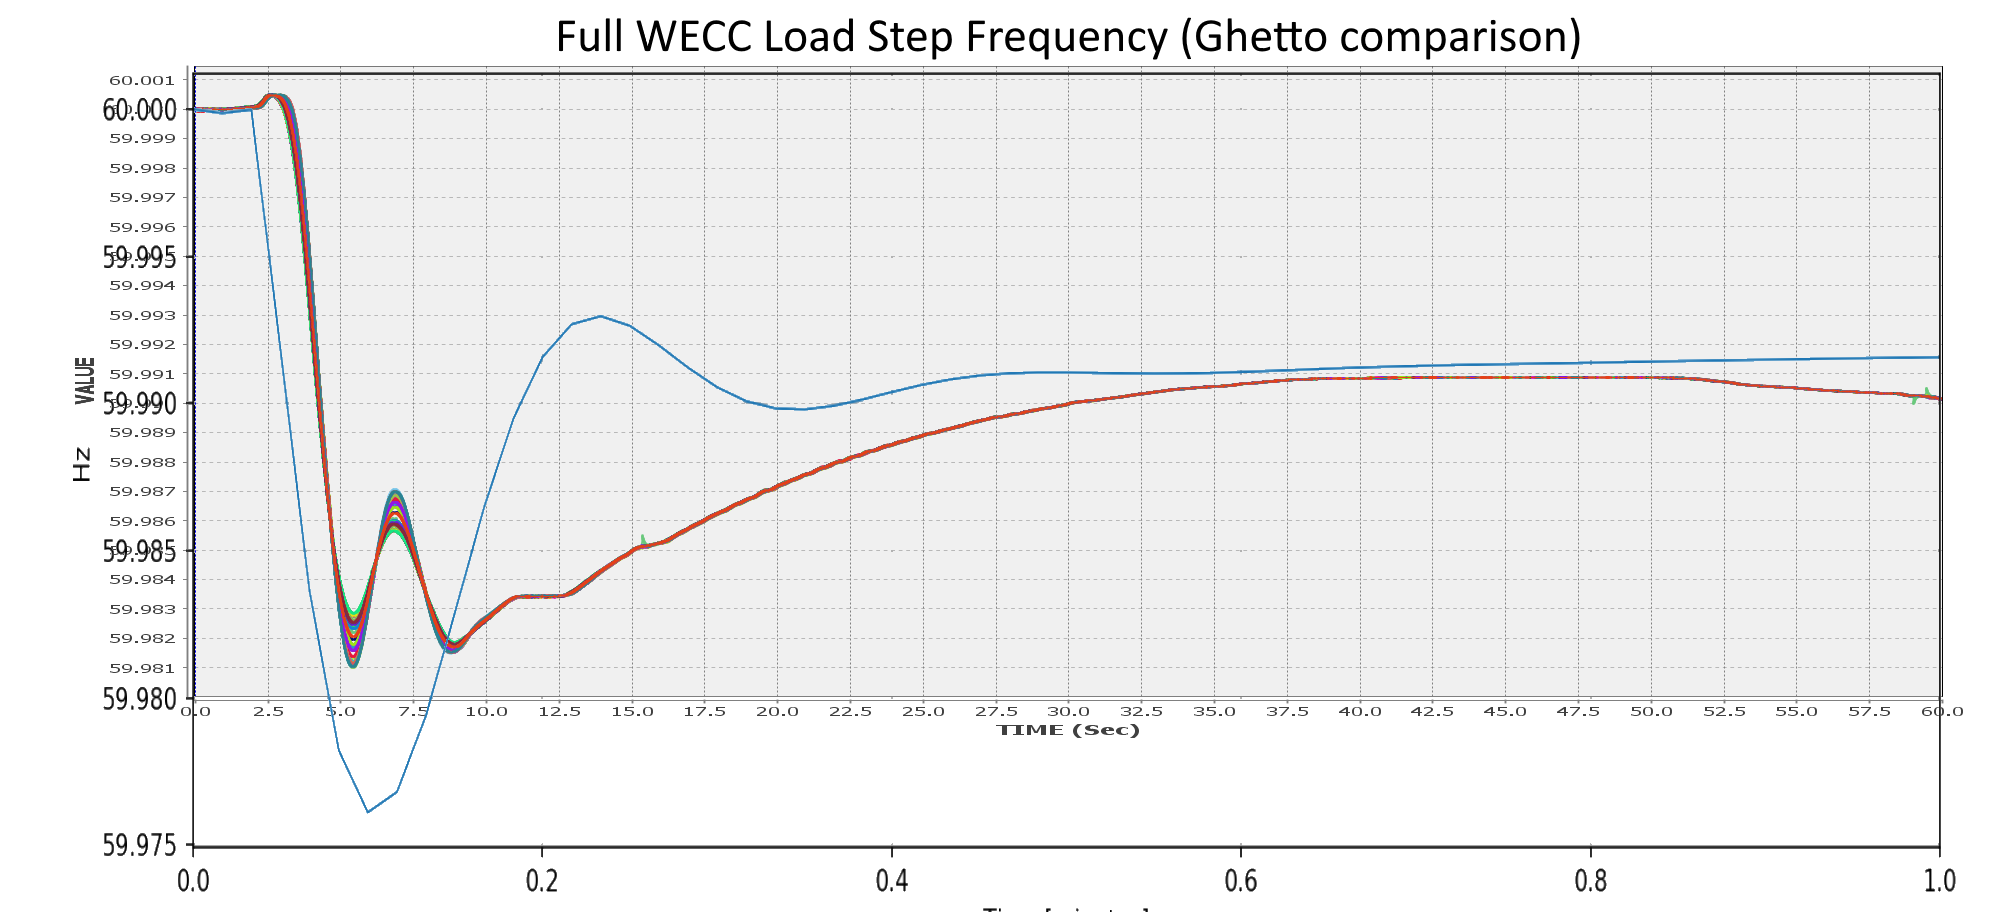
\includegraphics[width=\linewidth]{figures/weccStep}

The LTD software models only 20 tgov1 models with time constants from the dyd out the total 2,243 governors present (i.e. less than 1\% of LTD governors have the same time constants as PSDS).

From the frequency response, it is assumed that there are many more governors with hydro characteristics in the WECC dyd than are cast in the LTD simulation.
%\paragraph{'Soft Goals':}
%	\begin{enumerate}
%	\item Write Thesis 2020
%	\end{enumerate}

\pagebreak
% code
\paragraph{Initial DTC BPA results} Attempt at recreating GDACS control phenomena via given machine output.
Six machine system used, results show that method used not exactly correct.
Initial thought is that $\Delta \omega$ applied `twice' to Pref.

% results...
\begin{minipage}{.49\linewidth}
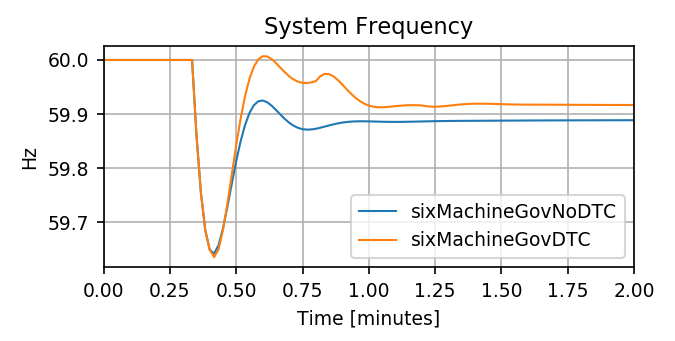
\includegraphics[width=\linewidth]{figures/f}
\end{minipage}%
\begin{minipage}{.49\linewidth}
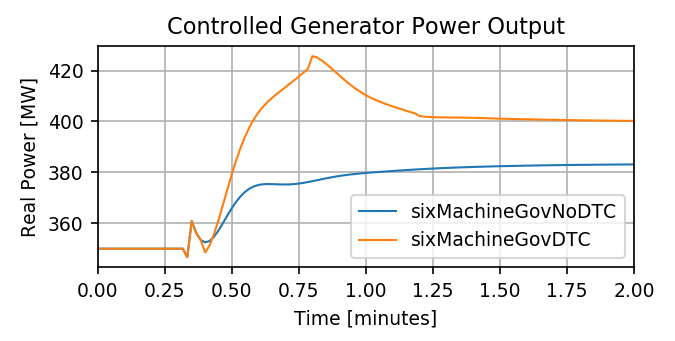
\includegraphics[width=\linewidth]{figures/pe}
\end{minipage}
\centering
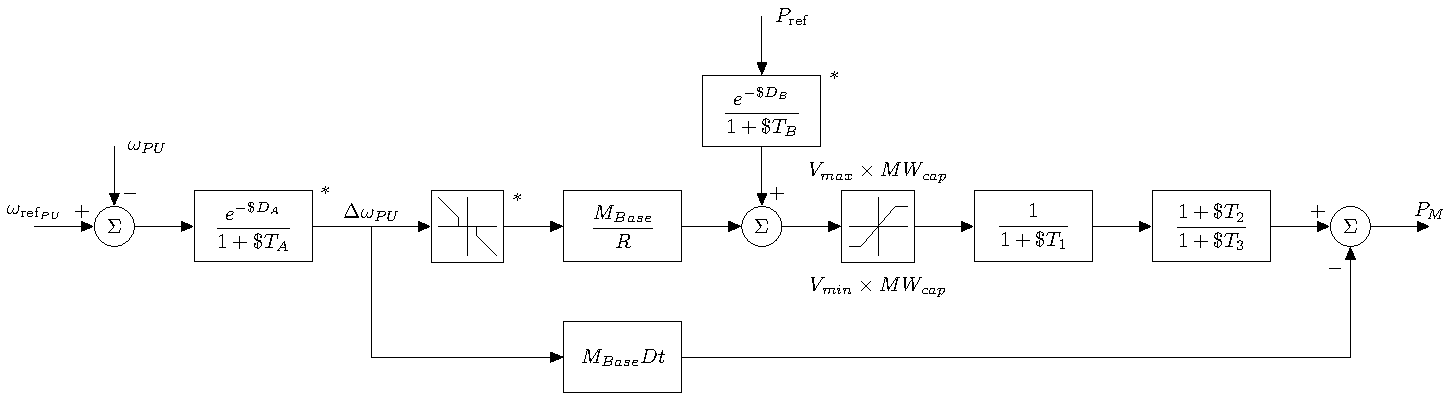
\includegraphics[width=.8\linewidth]{../../models/tgov1/tgov1DBdelay}

\begin{lstlisting}[language=Python]
# Perturbances
mirror.sysPerturbances = [
    'gen 5 : step Pm 20 -100 rel', # Step generator down
    ]

# Definite Time Controller Definitions
mirror.DTCdict = {
    'bpaTest' : {
        'RefAgents' : {
            'ra1' : 'mirror : f',
            'ra2' : 'gen 2 1 : R', 
            'ra3' : 'gen 2 1 : Pref0',
            'ra4' : 'gen 2 1 : Mbase',
            },# end Referenc Agents
        'TarAgents' : {
            'tar1' : 'gen 2 1 : Pref',
            }, # end Target Agents
        'Timers' : {
            'set' :{ # set Pref
                'logic' : "(ra1 > 0)", # should always eval as true
                'actTime' : 24, # seconds of true logic before act
                'act' : "tar1 = ra3 + (1-ra1)/(ra2) * ra4  ", # step 
                #'act' : "tar1 +=  (1-ra1)/ra2 * ra4 ", # step 
            },# end set
            'reset' :{ # not used
                'logic' : "0",
                'actTime' : 30, # seconds of true logic before act
                'act' : "0", # set any target On target = 0
            },# end reset
            'hold' : 0, # minimum time between actions
            }, # end timers
        },# end bpaTest
    }# end DTCdict

\end{lstlisting}
\end{document}